% !TEX root = ../oddp.tex

\section{A higher cup-product map}

In this section we build, from a certain equivariant map between spheres, a chain homomorphism with coefficients in $\bZ[\frac{1}{\tilde{r}!}]$.
\[\Psi\colon \hat{W}^*(r)\otimes N^r_*(\Delta^n)\to \bar{\Omega}^*(r,n)\]
Let $\Omega_*(r,m)$ be generated in degree $q$ by equivalence classes of generators $(U,w)\in \NN_*(\Delta^m\times EC_r)$ such that $w$ has at most one full piece, with the relation generated by inner reorderings. The differential $\sum_{i} (-1)^i(d_iU,d_iw)$ is well-defined in classes. $\Omega_*(r,m)^{nf}$ is the subcomplex of pairs without full pieces and $\Omega_*(r,m)^{f}$ is the submodule of pairs with full pieces.

Let $\Phi\colon \Omega_*(r,m)^f\to \Sigma^{r}\Omega_{*}(r,m-1)^{nf}$ be the (non-chain) homomorphism that sends a pair $(U,w)$ to the result of removing the full piece and decrease by one all entries in $U$ to the right of the piece, and increase by one all entries in $w$ to the right of the piece. It is endowed with the sign $(-1)^{\nu_i(U)}$ if the full piece restricts to the sequence $i=i=\ldots=i$ in $U$.

\begin{remark}
	 $\Phi^{\vee}(U,w) = \sum_i(-1)^{\nu_i(U)}D_i(U,w)$.
\end{remark}

\begin{lemma} \label{lemma:omegarm}
	Suppose given a family of $C_r$-equivariant homomorphism
	\begin{align*}
		\hat{\Psi}_*^m\colon \Omega_*(r,m)^{nf}&\lra \WW_*(r)
	\end{align*}
	related by the following equation:
	\begin{align}\label{it:1a}
		\hat{\Psi}^m_{q-1}((\partial (U,w)^{nf}) &= (-1)^{q-1}\hat{\Psi}^{m-1}_{q-r}\Phi(U,w) &\text{if $(U,w)$ has a full piece.}
	\end{align}
	%\begin{enumerate}
	%\item\label{it:1} $\hat{\Psi}_q\partial = \partial \hat{\Psi}_q + \hat{\Psi}_{q-r}\Phi$ !!!
	%\item\label{it:1a} $\hat{\Psi}_{q-1}((\partial (U,w)^{nf}) = \hat{\Psi}_{q-r}\Phi(U,w)$ if $w$ has a full piece.
	%\item\label{it:2a} $\hat{\Psi}_{q-1}((\partial (U,w)) = \partial \hat{\Psi}_{q}( (U,w))$ if $w$ has no full pieces.
	%\item\label{it:2} $\Phi(S_m(U,w)) = S_{m}(\Phi(U,w))$
	%\item\label{it:3} $\hat{\Psi}S_{m-1}\partial = \hat{\Psi}\partial S_m$ if $w$ has no full pieces
	%\item\label{it:4} $\hat{\Psi}_{r-2} = \theta_{r-1}\hat{\Psi}_{-1}S_{r-2}$
	%\end{enumerate}
	%Then $\hat{\Psi}$ extends recursively to the whole $\Omega_*(r,m)^{nf}$ as
	%\[
	%\hat{\Psi}_q =\begin{cases}
	%\hat{\Psi}_q & \text{if $q\leq r-2$} \\
	%\theta_{r-1}\hat{\Psi}_{q-r+1}S & \text{if $q\geq r-2$}.
	%\end{cases}
	%\]
	%and satisfies \eqref{it:1} and \eqref{it:3}, and
	Then there is a chain homomorphism
	\[\Psi\colon \WW^*(r)\otimes N^r_*(\Delta^n)\lra \Theta^*(r,n)\]
	defined as $\Psi(e_q\otimes \vec{\tau}) = (\hat{\Psi}^m)^\vee(e_q)\otimes \vec{\tau}$ if $\tau$ has dimension $m$.
\end{lemma}

\begin{proof}
	\begin{align*}
		\delta\hat{\Psi}^{\vee}(e_q)\otimes \vec{\tau}
		&= (\delta\hat{\Psi}^{\vee}(e_q))^{nf}\otimes\vec{\tau} + (\delta\hat{\Psi}^{\vee}(e_q))^f\otimes\vec{\tau} \\
		&= \hat{\Psi}^{\vee}(\delta e_q)\otimes \vec{\tau} +(-1)^q \Phi^\vee\check{\Psi}^\vee_{q-r+1}(e_{q-r+1})\otimes\vec{\tau} \\
		&= \hat{\Psi}^{\vee}(\delta e_{q})\otimes \vec{\tau} + (-1)^q \sum_i (-1)^{\nu_i(-)} D_i(\check{\Psi}^\vee_{q-r+1}(e_{q-r+1}))\otimes \vec{\tau}\\
		&= \hat{\Psi}^{\vee}(\delta e_q)\otimes \vec{\tau} + (-1)^q \sum_i \check{\Psi}^\vee_{q-r+1}(e_{q-r+1})\otimes d_i\vec{\tau} \\
		&= \Psi(\delta(e_q\otimes \vec{\tau}))\qedhere
	\end{align*}
\end{proof}

A \emph{pieced word} $w$ is a word in $EC_r$ together with a decomposition of $w$ into consecutive pieces of length $\leq r$. A \emph{full piece} is a piece of length $r$. Define the following relation on them:
\begin{itemize}
	\item (Inner reorderings) $w\sim (-1)^{|\sigma|}w'$ if all entries of $w$ and $w'$ coincide, except for a single piece where they differ by a permutation $\sigma$.
	%\item (Full piece removal) $w\sim (-1)^rw'$ if $w'$ is obtained from $w$ by removing a piece of length $r$ (a \emph{full piece}).
	\item (Standarization) $w\sim w'$ if $w'$ is obtained from $w$ by removing a piece of length $0$.
\end{itemize}
The complex $\Omega_*(r)$ is generated in degree $q$ by the equivalence classes of words of length $q+1$ and at most one full piece.
%Up to inner reorderings, every class $[w]$ has a maximal representative $\bar{w}$.
%Define $\partial([w]) = [\partial(\bar{w})]$.
The differential $\partial(w) = \sum_{i} (-1)^id_iw$ is well-defined in classes. $\Omega_*(r)^{nf}$ is the subcomplex of words without full pieces and $\Omega_*(r)^{f}$ is the submodule of words with full pieces.

If $(U,w)$ is a generator of $\Omega_*(r,m)$, then $w$ has a canonical piece decomposition: a sequence $(w_i,\ldots,w_{i+k})$ is a piece if and only if $u_{i-1}<u_i =\ldots= u_{i+k}<u_{i+k+1}$. This defines a chain homomorphism
\[\lambda_m\colon \Omega_*(r,m)\to \Omega_*(r)\]
Let $\Phi\colon \Omega_*(r)^f\to \Sigma^{r}\Omega_{*}(r)^{nf}$ be the (non-chain) homomorphism that sends a pieced word $w$ to the result of removing a full piece if it is possible and increase by one all entries in $w$ to the right of the piece. It has a sign given by $(-1)$ to the power of the number of entries to the right of the full piece. 
\begin{example}\label{ex:106}
    $\lambda_6([001123345566,012010212012]) = 01|20|1|02|1|20|12$
\end{example}

%If $w'$ is a subword of $w$ and $(U,w)$ is a pair, define the pair $(U|_{w'},w')$ in the obvious way.
%where $w^{*}=w$ if $w$ has no full piece and $0$ otherwise and $w^{**}$ is the opposite.

%A pieced word $w$ and a generator $U\in C^q(\Delta^m)$ are \emph{compatible} if they have the same length and if and only if the sequence $(w_i,\ldots,w_{i+k})$ is a piece. If $U$ and $w$ are compatible, write $(U,w)$ for the generator of $\hat{\Omega}^*(r,m)$ that is obtained by forgetting the pieces of $w$. Otherwise, define $(U,w) = 0$.

\begin{lemma} \label{lemma:omegar}
	Suppose one is given a $C_r$-equivariant chain homomorphism
	\begin{align*}
		\check{\Psi}\colon \Omega_*(r)^{nf}&\lra \WW_*(r)
	\end{align*}
	such that
	\begin{itemize}
		\item $(\tilde{r}!)\check{\Psi}_{q-1}((\partial (w)^{nf}) = (-1)^{q-1} \check{\Psi}_{q-r}\Phi(w)$ if $w$ has a full piece.
	\end{itemize}
	Then the family of maps $\hat{\Psi}^m = (\tilde{r}!)^m\check{\Psi}\lambda_m$ satisfies the conditions of Lemma \ref{lemma:omegarm}.
\end{lemma}

\begin{proof}
	Immediate.
\end{proof}

\subsection{Maps between spheres}\footnote{Actually we will need the map on unnormalised chains}

We will use the canonical identification $N_*(X*Y) \cong N_*(X)\otimes N_*(Y)$ and write $\sigma$ for the top dimensional class of $N_*(\Delta^{r-1})$. The cyclic group $C_r$ acts on $\Delta^{r-1}$ by permuting its vertices.
Let
\begin{align*}
	\iota_1\colon N_k(\Sigma^{r-1}\partial \Delta^{r-1})&\lra N_{k}(\partial\Delta^{r-1})\otimes N_{r-2}(\partial\Delta^{r-1})\\
	\iota_2\colon N_k(\Sigma^{r-1}\partial \Delta^{r-1})&\lra N_{r-2}(\partial\Delta^{r-1})\otimes N_{k}(\partial\Delta^{r-1})
\end{align*}
be the $C_r$-equivariant chain homomorphisms given by (here the simplices in $\partial \sigma$ have to be taken with the induced orientation)
\begin{align*}
	\iota_1(\tau) &= \tau\otimes \partial \sigma &
	\iota_2(\tau) &= \partial \sigma\otimes \tau 
\end{align*}
Let $f\colon N_*(\partial\Delta^{r-1}*\partial\Delta^{r-1})\to N_*(\mathbb{S}^{r-1}*\partial\Delta^{r-1})$ be a $C_r$-equivariant chain homomorphism such that
\renewcommand{\theenumi}{\roman{enumi}}
\begin{enumerate}
	\item\label{cond:1} $f\circ \iota_1 = \Id$
	\item\label{cond:2} $f\circ \iota_2 = \rho$.
	\item\label{cond:3} If $\tau_1\otimes\tau_2$ has degree $r-1$, then $f(\tau_1\otimes \tau_2)$ is a vertex if $\tau_1,\tau_2$ form a permutation and $0$ otherwise.
\end{enumerate}

\begin{remark}
	If we additionally impose the condition that $f$ sends simplices to simplices, then it is determined by its values on $(r-1)$-simplices.
\end{remark}

\begin{remark}
	Condition \eqref{cond:3} can be replaced by the more general condition
	\[
	\partial f(\tau_1\otimes\tau_2) =
	\begin{cases}
	\emptyset & \text{if $\tau_1$ and $\tau_2$ form a full permutation} \\
	0 & \text{otherwise}.
	\end{cases}
	\]
\end{remark}

%\begin{remark}
%	The former condition $f(\tau_1,\tau_2)\subset \tau_1$ is no longer necessary: It is necessary to define suspension maps for $\Omega_*(r,m)$, but with the current argument that is not needed.
%\end{remark}

%\begin{remark}
%	In the examples constructed, $f(\tau_1,\tau_2)\subset \tau_1\smallsetminus \tau_2$.
%\end{remark}

A word $w$ can be canonically broken into overlapping subwords of length at most $r$ called \emph{blocks}: Set the last block to be the last $r$ entries of the word, and recursively define the rest of the blocks by removing the last $r-1$ entries of the last block. Each pair of adjacent blocks share an element, that is called \emph{pivot}. All blocks have length $r$ except the first one, that has length strictly smaller than $r$. If $w$ is a minimal pieced word, let $w_1$ be the piece that contains the last pivot and let $w_2$ be the complement of that piece in the last block.

\begin{example}
	If $r=5$, the pieced word $w=01|24|013|12|4$ has as blocks $01-12401-13124$, the last pivot is $1$, and $w_1 = 013$ and $w_2 = 124$. If $r=3$, the pieced word $01|20|1|02|1|20|12$ has blocks $01-120-010-021-120-012$. Observe that the block decomposition is not unique, and depends on the representative. Nonetheless, the piece that contains the pivot is well-defined.
\end{example}

\begin{definition}
	Define a homomorphism $S\colon \Omega_*(r)^{nf}\to \Sigma^{r-1}\Omega_*(r)^{nf}$ by sending a pieced word $w$ to the result of replacing $w_1$ and $w_2$ by the piece $f(w_1,w_2)$. %If $w$ is a pieced word with a full piece, define $S(w)$ as the result of inserting back the full piece into $S(\Phi(w))$ (if the full piece was to the right of $w_1$, then it gets inserted at the end of the word).
\end{definition}

\begin{lemma}
	$S$ is a chain homomorphism.
\end{lemma}

\begin{proof}
	Let $\hat{w}$ be the result of removing $w_1$ and $w_2$ from $w$, and let $\ell$ be the degree of $\hat{w}$ (which is the same as the its cardinality). Given two words $w$ and $w'$, let $w*w'$ be its concatenation. Recall that $\partial w = \sum_{i} (-1)^{i}d_iw$, where $d_i$ removed the $i$-th entry of $w$. Then
	\begin{equation}\label{eq:931}
		\partial S(w) = \partial \hat{w}*f(w_1,w_2) + (-1)^{\ell}\hat{w}*\partial f(w_1,w_2).
	\end{equation}
	while, if the piece of the pivot contains at least two elements of the penultimate block,
	\[S(\partial w) = \partial \hat{w}*f(w_1,w_2) + (-1)^{\ell}\hat{w}*f(\partial(w_1),w_2) + (-1)^{\ell}\hat{w}*f(w_1,\partial w_2),\]
	which equals the previous sum. Suppose that the piece of the pivot is contained in the last block, in which case $f(w_1,w_2)$ is of dimension $0$. Then, letting $w_0$ be the piece to the left of $w_1$ and $\check{w}$ be the subword to the left of $w_0$, we have
	\begin{equation}\label{eq:933}
		S(\partial w) = \partial \hat{w}*f(w_1,w_2) + (-1)^\ell \check{w}*f(w_0,\partial(w_1*w_2)).
	\end{equation}
	Now, the last summand of \eqref{eq:931} is zero or $\hat{w}$ depending on whether $f(w_1,w_2)$ vanishes or not. By condition \eqref{cond:3}, this is equivalent to $w_1,w_2$ not being or being a full permutation, which by condition \eqref{cond:1} is equivalent to $f(w_0,\partial(w_1*w_2))$ being $0$ or $w_0$, and therefore equivalent to the last summand of \eqref{eq:933} being zero or $\hat{w}$.
\end{proof}

There is an inclusion $\CC_*(EC_r)\to \Omega_*(r)^{nf}$ that sends a word to that same word with all pieces of length $1$. There is a map in the opposite direction with $\bZ[\frac{1}{(r-1)!}]$-coefficients that sends a pieced word to the sum of the underlying words of all its representatives, divided by the number of representatives (there is a sign ambiguity due to the sign of the inner reorderings). The composition (here $\Psi$ is the map from the previous section)
\begin{equation} \label{eq:234}
	\Omega_*(r)^{nf}\lra C_*(EC_r)\overset{\Psi^\vee}{\lra} W_*(r)
\end{equation}
is a chain homomorphism with $\bZ[\frac{1}{(r-1)!}]$-coefficients (and the sign ambiguity due to inner reorderings disappears), but in degrees $*\leq r-2$ it lifts to a homomorphism with $\bZ$-coefficients, that we denote by $\check{\Psi}_*\colon \Omega_*(r)^{nf}\to W_*(r)$.

\begin{definition}
	Define a homomorphism $\check{\Psi}\colon \Omega_*(r)^{nf}\to W_*(r)$ recursively as
	\[\check{\Psi}_q(w) = \begin{cases} \check{\Psi}_q(w) & \text{if $*\leq r-2$} \\
		\frac{1}{\tilde{r}!}\theta_{1-r}\check{\Psi}_{q-r+1}S(w) & \text{if $*\geq r-2$.}\end{cases}\]
\end{definition}

\begin{lemma}
	$\check{\Psi}$ is a well-defined homomorphism. %$\check{\Psi}\partial = \partial\check{\Psi}$
\end{lemma}

\begin{proof}
	In degrees $*\leq r-2$ it is a homomorphism because it is a composition of the homomorphisms \eqref{eq:234}. The verification in the higher degrees follows from the previous lemma and induction (for clarity, we omit the factor $\frac{1}{\tilde{r}!}$):
	\begin{align*}
		\check{\Psi}_{q-1}\partial(w) &= \theta_{1-r}\check{\Psi}_{q-r}S\partial(w) = \theta_{1-r}\check{\Psi}_{q-r}\partial S(w) = \\
		&=\theta_{1-r}\partial\check{\Psi}_{q-r+1}S(w) = \partial\theta_{1-r}\check{\Psi}_{q-r+1}S(w) = \partial \check{\Psi}_{q}(w).
	\end{align*}
	Finally, recall that the map $\Psi_{r-2}$ of the previous section has a factor of $\frac{1}{\tilde{r}!}$ and consists on all permutations of $\{0,1,\ldots,r-1\}$, hence one deduces from \eqref{cond:3} that $\frac{1}{\tilde{r}!}\theta_{r-1}\check{\Psi}_{-1}S(w) = \check{\Psi}_{r-2}(w)$, hence both definitions coincide at their common case.
\end{proof}

%\begin{lemma} $\hat{\Psi}_{q-1}((\partial w)^{nf}) = \partial\hat{\Psi}_{q-r}\Phi(w)$ if $w$ has a full piece.
%\end{lemma}
%\begin{proof}
%\begin{itemize}
%\item if the full piece is to the left of $w_1$ \fcnote{doublecheck this, if it is exactly to the left an additional argument may be needed}, then $S\partial(w) = \partial S(w)$.
%\item if the full piece is to the right of $w_1$, then let $w_3$ be that full piece, and assume, without loss of generality that is the last piece. Then
%\[\partial S(w) = \partial \hat{w}*f(w_1,w_2)*w_3 + \hat{w}*\partial f(w_1,w_2)*w_3 + \hat{w}*f(w_1,w_2)*\partial w_3\]
%\[S\partial(w) = \partial \hat{w}*f(w_1,w_2)*w_3 + \hat{w}*\partial f(w_1,w_2)*w_3 + \hat{w}*w_1*f(w_2,\partial w_3)\]
%We need to check that the value of $\check{\Psi}$ in the last term coincides. If $q-r+1\geq r-2$, then we have that
%\[\check{\Psi}(\hat{w}*f(w_1,w_2)*\partial w_3) = \check{\Psi}S(\hat{w}*f(w_1,w_2)*\partial w_3) = \check{\Psi}(\hat{w}*f(f(w_1,w_2),\partial w_3)\]
%\[\check{\Psi}(\hat{w}*w_1*f(w_2,\partial w_3)) = \check{\Psi}S(\hat{w}*w_1*f(w_2,\partial w_3)) = \check{\Psi}(\hat{w}*f(w_1*f(w_2,\partial w_3))\]
%and both terms equal $f(w_1,w_2)$.
%\end{itemize}
%
%\end{proof}

\begin{lemma}
	$\tilde{r}!\check{\Psi}_{q-1}((\partial w)^{nf}) = (-1)^{q-1}\theta_{1-r} \check{\Psi}_{q-r}\Phi(w)$ if $w$ has a full piece.
\end{lemma}

\begin{proof}
	We will prove it by induction on the position from the right of the left piece. Since $w$ has at least one full piece, $q\geq r-1$ (for clarity, we omit the factor $\frac{1}{\tilde{r}!}$).

	If the full piece is the last piece, write $w=\hat{w}*w_1*w_2$ with $w_2$ the full piece. Then by Condition \eqref{cond:1}:
	%\[\partial S(w) = \partial \hat{w}*f(w_1,w_2)*w_3 + \hat{w}*\partial f(w_1,w_2)*w_3 + \hat{w}*f(w_1,w_2)*\partial w_3\]
	\begin{align*}
	    \tilde{r}!\theta_{1-r}\check{\Psi}_{q-1}((\partial w)^{nf}) &=
		\theta_{1-r}\check{\Psi}_{q-r}(S(\partial(w))^{nf}) \\
		&= (-1)^{q-r} \theta_{1-r}\check{\Psi}_{q-r}(S(\hat{w}*w_1*\partial w_2)) \\
		&= (-1)^{q-r} \theta_{1-r}\check{\Psi}_{q-r}(\hat{w}*f(w_1,\partial w_2)) \\
		&= (-1)^{q-1} \theta_{1-r}\check{\Psi}_{q-r}(\hat{w}*w_1) \\
		&= (-1)^{q-1} \theta_{1-r}\check{\Psi}_{q-r}\Phi(w).
	\end{align*}
	If the full piece is not the last piece but contains the pivot, write $w=\hat{w}*w_1*w_2$ with $w_1$ the full piece. Then by Condition \eqref{cond:2}:
	\begin{align*}
	    \tilde{r}!\theta_{1-r}\check{\Psi}_{q-1}((\partial w)^{nf}) &=
        \theta_{1-r}\check{\Psi}_{q-r}(S(\partial(w))^{nf}) \\&= \theta_{1-r}\check{\Psi}_{q-r}(S(\hat{w}*\partial w_1* w_2)) \\
		&= (-1)^{q-r} \theta_{1-r}\check{\Psi}_{q-r}(\hat{w}*f(\partial w_1, w_2)) \\
		&= (-1)^{q-1} \theta_{1-r}\check{\Psi}_{q-r}(\hat{w}*\rho(w_2)) \\
		&= (-1)^{q-1} \theta_{1-r}\check{\Psi}_{q-r}\Phi(w).
	\end{align*}
	If the full piece $\bar{w}$ is left to the last pivot (hence $q\geq 2r$), write $w=\hat{w}_1*\bar{w}*\hat{w}_2*w_1*w_2$ with $w_1$ the piece that contains the last pivot and $w_2$ the word to the right of $w_1$. Assume by induction that the lemma holds when $\hat{w}*w_1*w_2$ is of smaller length. Then
	\begin{align*}
		\tilde{r}!\theta_{1-r}\check{\Psi}_{q-1}((\partial w)^{nf}) &=
\theta_{1-r}\check{\Psi}_{q-r}(S(\partial(w))^{nf}) \\ 
		&= \theta_{1-r}\check{\Psi}_{q-r}S(\hat{w}_1*\partial\bar{w}*\hat{w}_2*w_1*w_2)) \\
		&= \theta_{1-r}\check{\Psi}_{q-r}(\hat{w}_1*\partial\bar{w}*\hat{w}_2*f(w_1,w_2)) \\
		&= \theta_{1-r}\check{\Psi}_{q-2r+1}(S(\hat{w}_1*\partial\bar{w}*\hat{w}_2*f(w_1,w_2)))\\
	    &\overset{*}{=} (-1)^{q-r} \theta_{1-r}\check{\Psi}_{q-2r+1}(\Phi(\hat{w}_1*\hat{w}_2*f(w_1,w_2))) \\
		&= (-1)^{q-1} \theta_{1-r}\check{\Psi}_{q-2r+1}(\hat{w}_1*\rho(\hat{w}_2*f(w_1,w_2)))\\
		&= (-1)^{q-1} \theta_{1-r}\check{\Psi}_{q-r}(\hat{w}_1*\rho(\hat{w}_2*w_1*w_2))\\
		&= (-1)^{q-1}\theta_{1-r}\check{\Psi}_{q-r}(\Phi(w)). \qedhere
	\end{align*}
In the three cases the sign in $\Phi(w)$ appears because after removing a full piece of odd length $r$ the parity of the indices elements to the right of that full piece changes.
\end{proof}

\begin{corollary} Each map $f\colon N_*(\Delta^{r-1})\otimes N_*(\Delta^{r-1})\to N_*(\Delta^{r-1})$ satisfying conditions \eqref{cond:1}, \eqref{cond:2} and \eqref{cond:3} yields a chain homomorphism $\check{\Psi}$ satisfying the conditions of Lemma \ref{lemma:omegar}.
\end{corollary}

\subsection{The pair barycentric subdivision} Recall that the barycentric subdivision $\sd \Delta^n$ of the geometric simplex $\Delta^n$ has one vertex for each non-empty face of $\Delta^n$ and every ascending chain of simplices $\sigma_0\subset \sigma_1\subset\ldots \subset \sigma_n$ of $\Delta^n$ yields a simplex $(\sigma_0,\ldots,\sigma_n)$ of the barycentric subdivision. 

The \emph{pair barycentric subdivision} $\Psd \Delta^n$ of $\Delta^n$ is a cubulation of $\Delta^n$ with the same vertices as $\sd \Delta^n$ and one face for each pair $(a,b)$ of faces of $\Delta^n$ such that $b\subset a$. That face is the union of all the faces of the barycentric subdivision that correspond to ascending chains $b\subset \sigma_0\subset \ldots\subset \sigma_k\subset a$. 

Think of the vertices of a cube $2^m$ as the powerset of $\{1,\ldots,m\}$. The pair barycentric subdivision is a cubulation of the geometric simplex where a pair $(a,b)$ with $m=|b\smallsetminus a|$ corresponds to the cube
\[F_{a,b}\colon 2^{m}\to \Delta^n\]
given by $F_{a,b}(u_1,\ldots,u_i) = b\cup \{c_1,\ldots,c_i\}$ where $c=a\smallsetminus b$. The associated cochain complex has differential
\[\delta(a,b) = \sum_{i=0}^m (-1)^i((a,\delta^i_c b)-(\partial^c_i a,b)\]
where $\partial_i^c$ removes the $i$th element of $c$ and $\delta^i_c$ adds the $i$th element of $c$.


There is a homomorphism 
\[s_*\colon N_*(\Delta^n)\to N_*(\Psd \Delta^n)\]
that sends each cubical face to the sum of all simplicial faces contained in it. There is a homomorphism
\[N_*(\Psd \Delta^n)\lra N_*(\sd \Delta^n)\]
that sends each cubical face to the sum of all simplicial faces contained in it,
\begin{definition}
    A pair barycentric subdivision map is a map if polyhedra $h\colon \Psd \Delta^n\to \Delta^n$ such that $h_*\circ s_* = \Id$ and [SOMETHING ELSE?]
\end{definition}
There is a map
\[g\colon N_*(\Delta^{r-1}*\Delta^{r-1})\lra N_*(\Sigma^{r-1}\Psd \Delta^{r-1})\]
that sends a pair $(a,b)$ to the pair $(a,a\smallsetminus b)$ if $(a,b)$ is a full permutation WITH AN APPROPRIATE SIGN QUITE DIFFICULT TO FIGURE OUT, and to zero otherwise. This map sends $(a,\partial \sigma)$ to the sum (AGAIN, THE SIGNS ARE DIFFICULT TO UNDERSTAND) $(-1)^{|a|}\sum_{i=0}^{|a|}(-1)^i (a,a_i)$ and $(\partial \sigma, b)$ to the sum $\sum_{b\subset d_i\sigma}(-1)^i(d_i\sigma,b)$.

\begin{proposition}
    If $h\colon \Psd \Delta^{r-1}\to \Delta^{r-1}$ is a cyclic pair barycentric subdivision map such that for every face $a$ of $\Delta^{r-1}$
    \begin{align*}
        (-1)^{|a|}\sum_{i=0}^{|a|}(-1)^i (a,a_i) &= a &
        \sum_{b\subset d_i\sigma}(-1)^i(d_i\sigma,b) &= \rho(b)
    \end{align*}
    with $\sigma$ the top simplex of $\Delta^{r-1}$, then the composition $f = h\circ g$ satisfies the conditions \eqref{cond:1}, \eqref{cond:2}, \eqref{cond:3}.
\end{proposition}
\begin{proof}
    The chain complex of $\Psd \Delta^n$ is generated in degree $k$ by pairs $(a,b)$ as above, with differential $\partial(a,b) = (\partial a,b) + (-1)^{|a|}(a,\delta^\dagger b)$. In this sum any pair $(a',b')$ in which $b'\not\subset a'$ is understood as zero. 
\end{proof}
If $r=3$, there is a unique cyclic subdivision map $h\colon \Psd \partial \Delta^{2}\to \partial \Delta^2$ satisfying both conditions (we only indicate the value on a cyclic basis):
\begin{align*}
    h([0],[0]) &= [0] &
    h([01],[01]) &= [0] 
\end{align*}
It yields the following map $f$ (we only indicate the non-zero values in a cyclic basis):
\begin{align*}
f([0]\otimes [1,2]) &= [0] & 
f([0,1]\otimes [2])&=0 &
f([0,1]\otimes [2,0]) &= [0,1]
\end{align*}
\begin{example}\label{ex:107}
    Let us find the image of $01|20|1|02|1|20|12$ under $\Psi$:
    \begin{align*}
        \Psi_{12}(01|20|1|02|1|20|12) &= \theta_2\Psi_{10}(01|20|1|02|1|f([20]\otimes[12])) = \theta_2\Psi_{10}(01|20|1|02|1|20)
        \\ &= \theta_4\Psi_8(01|20|1|02|f([1]\otimes [20])) = \theta_4\Psi_8(01|20|1|02|1)
        \\ &= \theta_6\Psi_6(01|20|1|f([02]\otimes [1])) = \theta_6\Psi_6(01|20|1|2)
        \\ &= \theta_8\Psi_4(01|f([20]\otimes [12])) = \theta_8\Psi_4(01|20)
        \\ &= \theta_{10}\Psi_2(f([01]\otimes [20])) = \theta_{10}\Psi_2(01) 
        \\ &= e_{12}
    \end{align*}
\end{example}
\begin{figure}
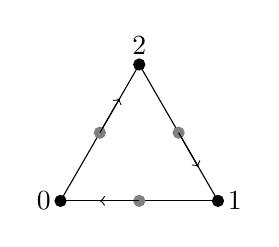
\begin{tikzpicture}
    \draw (0,1.732) -- (1,0);
    \draw (-1,0) -- (1,0);
    \draw (-1,0) -- (0,1.732);
    \filldraw [gray] (-.5,.866) circle (2pt);
    \filldraw [gray] (.5,.866) circle (2pt);
    \filldraw [gray] (0,0) circle (2pt);
    \filldraw [black] (0,1.732) circle (2pt)  node[anchor=south]{2};
    \filldraw [black] (1,0) circle (2pt) node[anchor=west]{1};
    \filldraw [black] (-1,0) circle (2pt) node[anchor=east]{0};
    \draw[->] (0,0) -- (-.5,0);
    \draw[->] (-.5,.866) -- (-.25,1.299);
    \draw[->] (.5,.866) -- (.75,.433);
\end{tikzpicture}
\caption{The cyclic subdivision map for $\partial \Delta^2$.}
\end{figure}

\begin{figure}
\begin{tikzpicture}[line join = round, line cap = round]
\pgfmathsetmacro{\factor}{1/sqrt(2)};
\coordinate [label=left:A] (A) at (-2,0,0);
\coordinate [label=below:B] (B) at (.4,-1,0);
\coordinate [label=right:2] (C) at (2,0,0);
\coordinate [label=above:3] (D) at (0,2.8,.2);

path (B) -- (C) node[midway] (BC) {BC}

\coordinate (AB) at $(A+B)/2$;
\coordinate (AC) at (0,0,0);
\coordinate (AD) at (2,0,0);
\coordinate (D) at (0,2.8,.2);

%\draw[->] (0,0) -- (3,0,0) node[right] {$x$};
%\draw[->] (0,0) -- (0,3,0) node[above] {$y$};
%\draw[->] (0,0) -- (0,0,3) node[below left] {$z$};
\foreach \i in {A,B,C,D}
    \draw[dashed] (\i) -- (AB);
\draw[-, fill=red!30, opacity=.5] (A)--(D)--(B)--cycle;
\draw[-, fill=green!30, opacity=.5] (A) --(D)--(C)--cycle;
\draw[-, fill=purple!30, opacity=.5] (B)--(D)--(C)--cycle;
\end{tikzpicture}
    \caption{The cyclic subdivision map for $\partial \Delta^4$ on the face $[0,1,2,3]$ (the other faces are in the $C_r$-orbit of this face).}
    \label{fig:my_label}
\end{figure}

If $r=5$, then there is a cyclic subdivision map $h\colon \Psd \partial \Delta^4\to \partial \Delta^4$ satisfying both conditions: 
\begin{align*}
    h([0],[0]) &= [0] &
	h([01],[01]) &= [0] &
	h([02],[02]) &= [0] \\
	h([012],[012]) &= [0] &
	h([013],[013]) &= [0] &
	h([0123],[0123]) &= [0]
\end{align*}
It yields the following map $f\colon N_*(\partial \Delta^4)\otimes N_*(\partial \Delta^4)\to \Sigma^4N_*(\partial \Delta^4)$ (again, we only indicate the non-zero values of $f$ on a cyclic basis):
\begin{align*}
	f([0]\otimes[1,2,3,4]) &= [0] &
	f([0,1]\otimes [2,3,4]) &= [0] \\
	f([0,2]\otimes [1,3,4]) &= [0] &
	f([0,1,2]\otimes [3,4]) &= [0] \\
	f([0,1,3]\otimes [2,4]) &= [0] &
	f([0,1,2,3]\otimes [4]) &= [0] \\
	f([0,1]\otimes [2,3,4,0]) &= [0,1] &
	f([0,2]\otimes [1,3,4,0]) &= [0,2] \\
	f([0,1,3]\otimes [2,4,0]) &= [0,1] &
	f([0,1,3]\otimes [2,4,1]) &= [0,3] \\
	f([0,1,2,3]\otimes [4,0]) &= [0,1] &
	f([0,1,2,3]\otimes [4,1]) &= [2,0] \\
	f([0,1,2]\otimes [3,4,0]) &= [0,1,2] &
	f([0,1,3]\otimes [2,4,0,1]) &= [0,1,3] \\
	f([0,1,2,3]\otimes [4,0,1]) &= [0,1,2] &
	f([0,1,2,3]\otimes [4,1,2]) &= [0,2,3] \\
	f([0,1,2,3]\otimes [4,0,1,2]) &= [0,1,2,3] 
\end{align*}
This map is not unique, the map obtained by redefining $h([013],[013]) = [3]$ also extends. 

If $r=7$, then there is a cyclic subdivision map $h\colon \Psd \partial \Delta^6\to \partial \Delta^6$ satisfying both conditions. Below are the vertices that map to the vertex $0$, which cyclically determine the map $h$:  
\begin{align*}
			(0) &&
			(0,1) &&
			(0,2) &&
			(0,3) \\
			(0,1,2) &&
			(0,1,3) &&
			(0,1,4) &&
			(0,2,3) &&
			(0,2,4) \\
			(0,1,2,3) &&
			(0,1,2,4) &&
			(0,1,3,4) &&
			(0,2,3,4) &&
			(0,1,3,5) \\
			(0,1,2,3,4) &&
			(0,1,2,3,5) &&
			(0,1,3,4,5) &&
			(0,1,2,3,4,5)
\end{align*}
It yields the following map $f\colon N_*(\partial \Delta^6)\otimes N_*(\partial \Delta^6)\to \Sigma^6N_*(\partial \Delta^6)$ (again, we only indicate the non-zero values of $f$ on a cyclic basis):
\begin{align*}
f( [0] \otimes [1, 2, 3, 4, 5, 6] )&= [0] &
f( [0, 1] \otimes [2, 3, 4, 5, 6] )&= [0] \\
f( [0, 2] \otimes [1, 3, 4, 5, 6] )&= [0] &
f( [0, 3] \otimes [1, 2, 4, 5, 6] )&= [0] \\
f( [0, 1, 2] \otimes [3, 4, 5, 6] )&= [0] &
f( [0, 1, 3] \otimes [2, 4, 5, 6] )&= [0] \\
f( [0, 1, 4] \otimes [2, 3, 5, 6] )&= [0] &
f( [0, 2, 3] \otimes [1, 4, 5, 6] )&= [0] \\
f( [0, 2, 4] \otimes [1, 3, 5, 6] )&= [0] &
f( [0, 1, 2, 3] \otimes [4, 5, 6] )&= [0] \\
f( [0, 1, 2, 4] \otimes [3, 5, 6] )&= [0] &
f( [0, 1, 3, 4] \otimes [2, 5, 6] )&= [0] \\
f( [0, 1, 3, 5] \otimes [2, 4, 6] )&= [0] &
f( [0, 2, 3, 4] \otimes [1, 5, 6] )&= [0] \\
f( [0, 1, 2, 3, 4] \otimes [5, 6] )&= [0] &
f( [0, 1, 2, 3, 5] \otimes [4, 6] )&= [0] \\
f( [0, 1, 3, 4, 5] \otimes [2, 6] )&= [0] &
f( [0, 1, 2, 3, 4, 5] \otimes [6] )&= [0] \\
f( [0, 1] \otimes [0, 2, 3, 4, 5, 6] )&= [0, 1] &
f( [0, 2] \otimes [0, 1, 3, 4, 5, 6] )&= [0, 2] \\
f( [0, 3] \otimes [0, 1, 2, 4, 5, 6] )&= [0, 3] &
f( [0, 1, 2] \otimes [0, 3, 4, 5, 6] )&= [0, 1] \\
f( [0, 1, 3] \otimes [0, 2, 4, 5, 6] )&= [0, 1] &
f( [0, 1, 4] \otimes [0, 2, 3, 5, 6] )&= [0, 1] \\
f( [0, 1, 4] \otimes [1, 2, 3, 5, 6] )&= [0, 4] &
f( [0, 2, 3] \otimes [0, 1, 4, 5, 6] )&= [0, 2] \\
f( [0, 2, 4] \otimes [0, 1, 3, 5, 6] )&= [0, 2] &
f( [0, 2, 4] \otimes [1, 2, 3, 5, 6] )&= [0, 4] \\
f( [0, 1, 2, 3] \otimes [0, 4, 5, 6] )&= [0, 1] &
f( [0, 1, 2, 4] \otimes [0, 3, 5, 6] )&= [0, 1] \\
f( [0, 1, 3, 4] \otimes [0, 2, 5, 6] )&= [0, 1] &
f( [0, 1, 3, 4] \otimes [1, 2, 5, 6] )&= [0, 3] \\
f( [0, 1, 3, 5] \otimes [0, 2, 4, 6] )&= [0, 1] &
f( [0, 1, 3, 5] \otimes [1, 2, 4, 6] )&= [0, 3] \\
f( [0, 1, 3, 5] \otimes [2, 3, 4, 6] )&= [0, 5] &
f( [0, 2, 3, 4] \otimes [0, 1, 5, 6] )&= [0, 2] \\
f( [0, 2, 3, 4] \otimes [1, 2, 5, 6] )&= [0, 3] &
f( [0, 1, 2, 3, 4] \otimes [0, 5, 6] )&= [0, 1] \\
f( [0, 1, 2, 3, 5] \otimes [0, 4, 6] )&= [0, 1] &
f( [0, 1, 2, 3, 5] \otimes [1, 4, 6] )&= [0, 2] \\
f( [0, 1, 2, 3, 5] \otimes [3, 4, 6] )&= [0, 5] &
f( [0, 1, 3, 4, 5] \otimes [0, 2, 6] )&= [0, 1] \\
f( [0, 1, 3, 4, 5] \otimes [1, 2, 6] )&= [0, 3] &
f( [0, 1, 3, 4, 5] \otimes [2, 3, 6] )&= [0, 4] \\
f( [0, 1, 2, 3, 4, 5] \otimes [0, 6] )&= [0, 1] &
f( [0, 1, 2, 3, 4, 5] \otimes [1, 6] )&= [0, 2] \\
f( [0, 1, 2, 3, 4, 5] \otimes [3, 6] )&= [0, 4] &
f( [0, 1, 2] \otimes [0, 1, 3, 4, 5, 6] )&= [0, 1, 2] \\
f( [0, 1, 3] \otimes [0, 1, 2, 4, 5, 6] )&= [0, 1, 3] &
f( [0, 1, 4] \otimes [0, 1, 2, 3, 5, 6] )&= [0, 1, 4] \\
f( [0, 2, 3] \otimes [0, 1, 2, 4, 5, 6] )&= [0, 2, 3] &
f( [0, 2, 4] \otimes [0, 1, 2, 3, 5, 6] )&= [0, 2, 4] \\
f( [0, 1, 2, 3] \otimes [0, 1, 4, 5, 6] )&= [0, 1, 2] &
f( [0, 1, 2, 4] \otimes [0, 1, 3, 5, 6] )&= [0, 1, 2] \\
f( [0, 1, 3, 4] \otimes [0, 1, 2, 5, 6] )&= [0, 1, 3] &
f( [0, 1, 3, 4] \otimes [1, 2, 3, 5, 6] )&= [0, 3, 4] \\
f( [0, 1, 3, 5] \otimes [0, 1, 2, 4, 6] )&= [0, 1, 3] &
f( [0, 1, 3, 5] \otimes [0, 2, 3, 4, 6] )&= [0, 1, 5] \\
f( [0, 1, 3, 5] \otimes [1, 2, 3, 4, 6] )&= [0, 3, 5] &
f( [0, 2, 3, 4] \otimes [0, 1, 2, 5, 6] )&= [0, 2, 3] \\
f( [0, 2, 3, 4] \otimes [1, 2, 3, 5, 6] )&= [0, 3, 4] &
f( [0, 1, 2, 3, 4] \otimes [0, 1, 5, 6] )&= [0, 1, 2] \\
f( [0, 1, 2, 3, 5] \otimes [0, 1, 4, 6] )&= [0, 1, 2] &
f( [0, 1, 2, 3, 5] \otimes [0, 3, 4, 6] )&= [0, 1, 5] \\
f( [0, 1, 2, 3, 5] \otimes [1, 2, 4, 6] )&= [0, 2, 3] &
f( [0, 1, 2, 3, 5] \otimes [1, 3, 4, 6] )&= [0, 2, 5] \\
f( [0, 1, 3, 4, 5] \otimes [0, 1, 2, 6] )&= [0, 1, 3] &
f( [0, 1, 3, 4, 5] \otimes [0, 2, 3, 6] )&= [0, 1, 4] \\
f( [0, 1, 3, 4, 5] \otimes [1, 2, 3, 6] )&= [0, 3, 4] &
f( [0, 1, 3, 4, 5] \otimes [2, 3, 4, 6] )&= [0, 4, 5] \\
f( [0, 1, 2, 3, 4, 5] \otimes [0, 1, 6] )&= [0, 1, 2] &
f( [0, 1, 2, 3, 4, 5] \otimes [0, 3, 6] )&= [0, 1, 4] \\
f( [0, 1, 2, 3, 4, 5] \otimes [1, 2, 6] )&= [0, 2, 3] &
f( [0, 1, 2, 3, 4, 5] \otimes [1, 3, 6] )&= [0, 2, 4] \\
f( [0, 1, 2, 3, 4, 5] \otimes [3, 4, 6] )&= [0, 4, 5] 
\end{align*}
\begin{align*}
f( [0, 1, 2, 3] \otimes [0, 1, 2, 4, 5, 6] )&= [0, 1, 2, 3] \\
f( [0, 1, 2, 4] \otimes [0, 1, 2, 3, 5, 6] )&= [0, 1, 2, 4] \\
f( [0, 1, 3, 4] \otimes [0, 1, 2, 3, 5, 6] )&= [0, 1, 3, 4] \\
f( [0, 1, 3, 5] \otimes [0, 1, 2, 3, 4, 6] )&= [0, 1, 3, 5] \\
f( [0, 2, 3, 4] \otimes [0, 1, 2, 3, 5, 6] )&= [0, 2, 3, 4] \\
f( [0, 1, 2, 3, 4] \otimes [0, 1, 2, 5, 6] )&= [0, 1, 2, 3] \\
f( [0, 1, 2, 3, 5] \otimes [0, 1, 2, 4, 6] )&= [0, 1, 2, 3] \\
f( [0, 1, 2, 3, 5] \otimes [0, 1, 3, 4, 6] )&= [0, 1, 2, 5] \\
f( [0, 1, 2, 3, 5] \otimes [1, 2, 3, 4, 6] )&= [0, 2, 3, 5] \\
f( [0, 1, 3, 4, 5] \otimes [0, 1, 2, 3, 6] )&= [0, 1, 3, 4] \\
f( [0, 1, 3, 4, 5] \otimes [0, 2, 3, 4, 6] )&= [0, 1, 4, 5] \\
f( [0, 1, 3, 4, 5] \otimes [1, 2, 3, 4, 6] )&= [0, 3, 4, 5] \\
f( [0, 1, 2, 3, 4, 5] \otimes [0, 1, 2, 6] )&= [0, 1, 2, 3] \\
f( [0, 1, 2, 3, 4, 5] \otimes [0, 1, 3, 6] )&= [0, 1, 2, 4] \\
f( [0, 1, 2, 3, 4, 5] \otimes [0, 3, 4, 6] )&= [0, 1, 4, 5] \\
f( [0, 1, 2, 3, 4, 5] \otimes [1, 2, 3, 6] )&= [0, 2, 3, 4] \\
f( [0, 1, 2, 3, 4, 5] \otimes [1, 3, 4, 6] )&= [0, 2, 4, 5] \\
f( [0, 1, 2, 3, 4] \otimes [0, 1, 2, 3, 5, 6] )&= [0, 1, 2, 3, 4] \\
f( [0, 1, 2, 3, 5] \otimes [0, 1, 2, 3, 4, 6] )&= [0, 1, 2, 3, 5] \\
f( [0, 1, 3, 4, 5] \otimes [0, 1, 2, 3, 4, 6] )&= [0, 1, 3, 4, 5] \\
f( [0, 1, 2, 3, 4, 5] \otimes [0, 1, 2, 3, 6] )&= [0, 1, 2, 3, 4] \\
f( [0, 1, 2, 3, 4, 5] \otimes [0, 1, 3, 4, 6] )&= [0, 1, 2, 4, 5] \\
f( [0, 1, 2, 3, 4, 5] \otimes [1, 2, 3, 4, 6] )&= [0, 2, 3, 4, 5] \\
f( [0, 1, 2, 3, 4, 5] \otimes [0, 1, 2, 3, 4, 6] )&= [0, 1, 2, 3, 4, 5] \\
\end{align*}

\begin{lemma}
    If $f\colon \partial \Delta^{r-1}*\partial\Delta^{r-1}\to \Sigma^{r-1}\partial \Delta^{r-1}$ is a $C_r$-equivariant map, then $r$ is prime.
\end{lemma}
\begin{proof}
    This is due to the fact that the action of $C_r$ of $\partial \Delta^{r-1}$ is always free, while the action of $C_r$ on the join is free only if $r$ is prime: if $r=pq$, then $\rho$ has order $q$ on the simplex $\tau_1 = [0,p,2p,\ldots,(q-1)p]$ and on its complementary simplex $\tau_2 = PD(\tau_1)$. Therefore $f(\rho^q(\tau_1,\tau_2)) = f(\tau_1,\tau_2)\neq \rho^q(f(\tau_1,\tau_2))$.
\end{proof}
\subsection{Symmetric comultiplications} Let $\mu\colon W_*(r)\otimes N_*(\Delta^n)\lra N_*(\Delta^n)^{\otimes r}$ be the composition $\mu = \mathrm{rev}\circ\alpha\circ\beta\circ\beta'\circ\Psi^{\vee}\circ\varphi$. Let $\mu_k\colon N_*(\Delta^n)\to N_*(\Delta^n)^{\otimes r}$ be defined as $\mu_k(\tau) = \mu(e_k\otimes \tau)$. 
\begin{theorem} Given a pair barycentric subdivision map $h$, the family $\{\mu_k\}$ is a symmetric comultiplication in $N_*(\Delta^n;\bZ)$. 
\end{theorem}
\federico{Here $\bZ$ coefficients are allowed because of the factor $(\tilde{r}!)^m$ in the definition of Lemma \eqref{lemma:omegar} that I did not notice until the very end}
\begin{example}
    From Examples \ref{ex:101},\ref{ex:102},\ref{ex:103},\ref{ex:104},\ref{ex:105},\ref{ex:106} and \ref{ex:107} we deduce that, for $r=3$, the coefficient of $[0,2,3]\otimes [3,4,5]\otimes [5,7,9]$ in $\mu_0([0,2,3,4,5,7,9])$ is $-1$.
\end{example}
Let us give a self-contained description of these comultiplication maps: Recall that the last pivot of a word $w = (w_0,\ldots,w_q)\in (EC_r)_q$ is the entry $w_{q-r+1}$. Recall that if $U\in C^q(\Delta^n)$ and $w\in C^q(EC_r)$ are generators, a piece in $w$ is a sequence $w_i,w_{i+1},\ldots,w_{i+l}$ such that $u_{i-1}<u_i = u_{i+1} = \ldots = u_{i+k} < u_{i+k+1}$. Write $w_1$ for the piece that contains the last pivot and $w_2$ for the part of $w$ to the right of $w_1$ and $\hat{w}$ for the part of $w$ to the left of $w_1$. Recall that a pieced word is a word with a decomposition into subwords of length $<r$.

\begin{definition} A pieced word $w$ of length $<r$ is \emph{admissible} if there is a permutation $\sigma$ such that $(w_{\sigma(0)},w_{\sigma(1)},\ldots,w_{\sigma(q)})$ is an increasing sequence and $w_{i}$ has the same parity as $i$. Its sign is the sign of the permutation $\sigma$.

For longer pieced words the definition is recursive: a word of length $\geq r$ is \emph{admissible} if $h(w_1,w_1\smallsetminus w_2)$ is non-zero and $\hat{w}*h(w_1,w_1\smallsetminus w_2)$ is admissible. The sign of $w$ is the product of the signs SIGNS OF THE MAP FROM THE JOIN TO THE BARYCENTRIC SUBDIVISION. 
\end{definition}
\begin{definition}
    A pair $(U,w)\in N^*(\Delta^n\times EC_r)$ is \emph{compatible} if the pieced word $w$ is admissible.
\end{definition}
\begin{definition}
    The \emph{sign} of a pair $(U,w)\in N^*(\Delta^n\times EC_r)$ is the product of the following signs:
    \begin{itemize}
    \item the sign of $w$.
    \item The sign of the permutation that orders $w$ [I have the impression that it almost cancels with the sign of w].
    \item $\mu(U_0,\ldots,U_{r-1},\tau)$
    \item $\lambda(U)$ (the sum of the entries of $U$)
    \item the sign of $\mathrm{rev}$. 
\end{itemize}
\end{definition}
\begin{example}
    ($r=3$) Recall that a word of length $2\ell+s$ in $EC_3$ has a canonical block decomposition into $\ell+1$ overlapping blocks, the first having length $s$ and the rest having length $3$. A block $(a_1,a_2,a_3)$ is \emph{ascending} if $a_2=a_1+1$ and $a_3=a_2+1$. A pieced word $w\in EC_3$ is \emph{admissible} if no block as repeated elements and every block containing a piece of length $2$ is ascending. The sign of $w$ is the number of non-ascending blocks in $w$.
\end{example}
The comultiplication map $\mu_k$ is given by
\[\mu_k(\tau) = \sum_{\begin{array}{c}\text{\footnotesize $(U,w)$ compatible }\\ \text{ \footnotesize of length $(r-1)m-k$}\end{array}} (-1)^{s(U,w)}(d_{U^{r-1}_{w}}(\tau)\otimes d_{U^{r-2}_{w}}(\tau)\otimes \ldots \otimes d_{U^{0}_{w}}(\tau) )\]

We have empirically found that our formulas coincide with the formulas in [ANIBAL] in arity $3$, and that they are different from the formulas in [ANIBAL] in arity $5$.
